% !TeX spellcheck = en_GB
\graphicspath{ {./diagrams/} }
\chapter{Other Design Considerations}\label{chapter:Other Design Considerations}

\section{Kernel Architecture}

\begin{flushleft}
	There are three types of kernel architectures:
		\begin{enumerate}
			\item \textbf{Micro Kernel}
			\item \textbf{Monolithic Kernel}
			\item \textbf{Hybrid Kernel}
		\end{enumerate}
	
	This classification is based on what is in kernel space and what is in user space. There are four
	protection rings that represent the access a piece of software has to the hardware and system. Out
	of these only two rings are of interest:
		\begin{enumerate}
			\item \textbf{Ring 0}\\
			Code running in Ring 0 is said to be in supervisor mode. It has complete access to the hardware
			and system.
			
			\item \textbf{Ring 3}\\
			Code running in Ring 3 is said to be in user space. It has no direct access to hardware or the
			system. Instead it accesses the system through syscalls.
		\end{enumerate}
	These protections are not simply implemented by the Operating system. Instead they are a part of
	the CPU architecture. They are activated by asm code.
	\begin{itemize}
		\item In a \textbf{micro kernel} very limited amount of code is is in kernel space. For example, most drivers are
		in userspace.
		\item In a \textbf{monolithic kernel} device drivers and other similar modules operate in kernel space.
		\item A \textbf{hybrid kernel} is somewhere in the middle of what runs in kernel space and user space.
	\end{itemize}

	Dax OS has a monolithic design. This is motivated by two facts which are:
	\begin{itemize}
		\item The Linux kernel is monolithic. Therefore if we use a micro kernel architecture, students will not be
		able to transfer the knowledge that they acquired from our project into the linux development space.
		
		\item Our kernel operates completely in ring-0 i.e without any restrictions. Implementing user-mode
		is unnecessary since we have no user-mode programs. Additionally students need to be in ring-0
		to understand how the hardware works.
		
	\end{itemize}
	
\end{flushleft}
\begin{figure}[h!]
	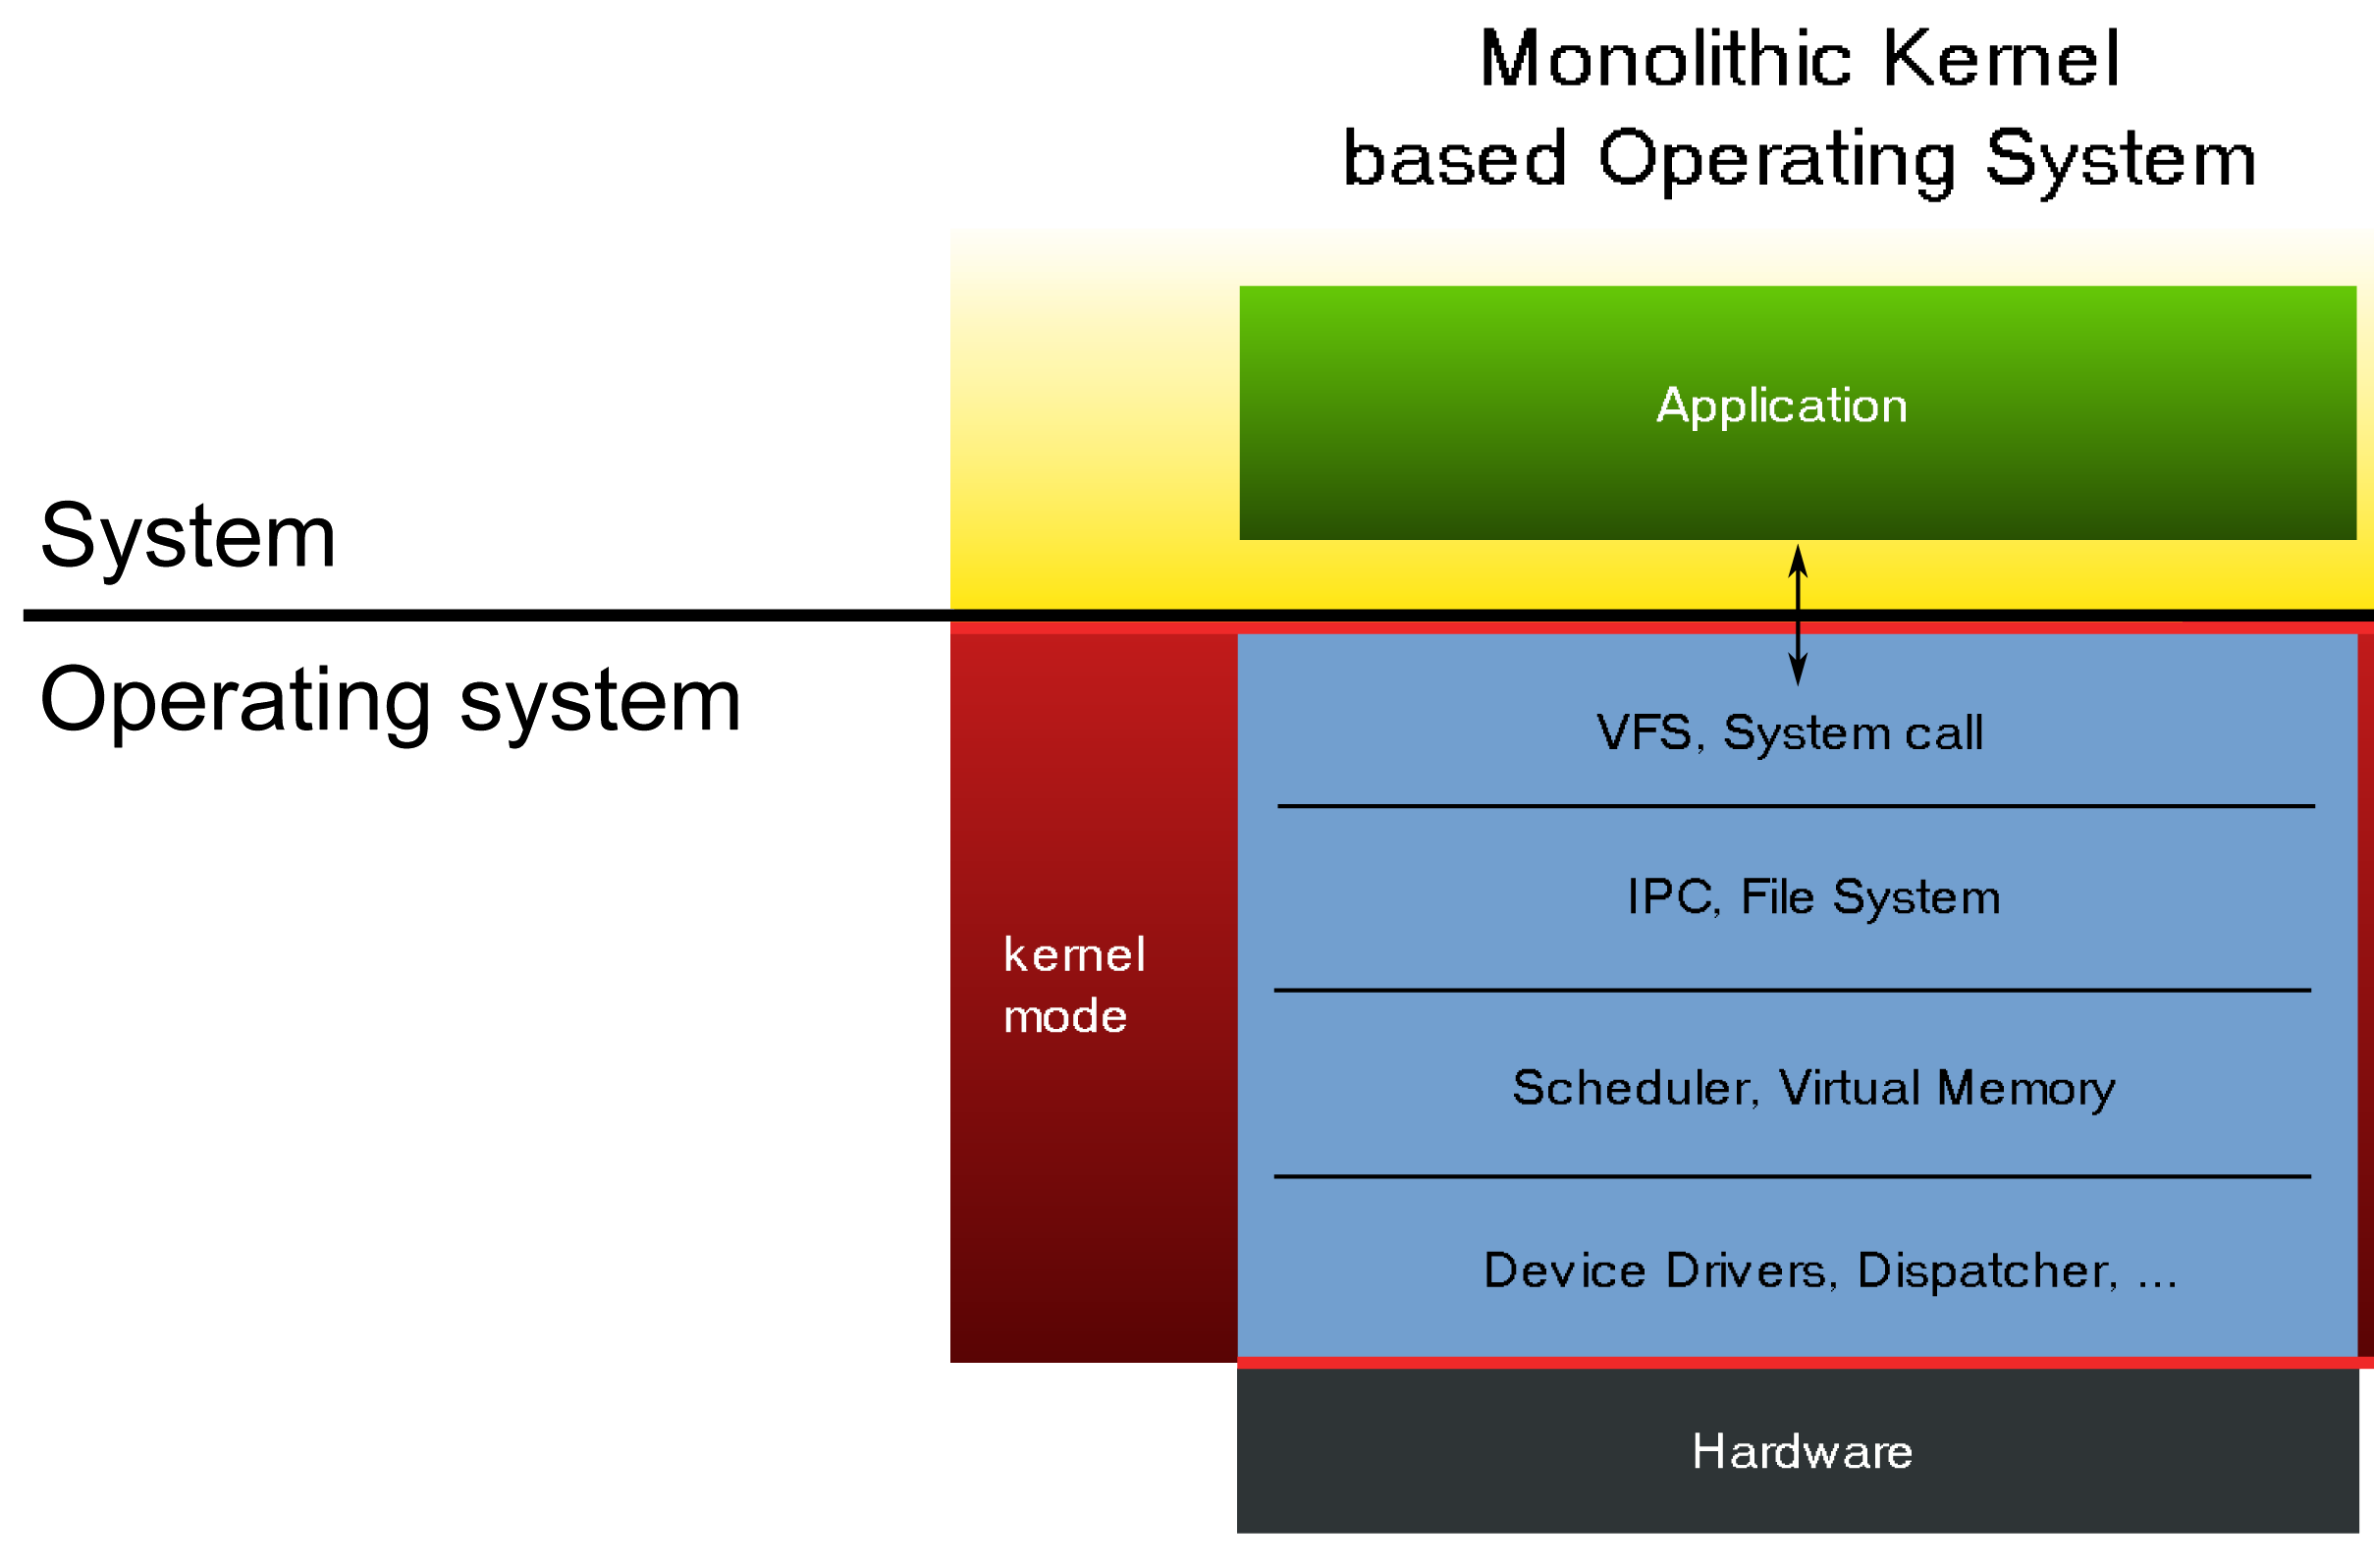
\includegraphics[width=\textwidth,height=\textheight,keepaspectratio]{kernel_arch}
	\caption{Illustration of Kernel Architecture}
\end{figure}
\pagebreak

\section{Build Process}
\begin{flushleft}
	The build architecture is a little involved because the C programming language
	does not have any real tooling for package management. Instead compiling and linking
	each translation unit must be done manually.
	\vspace{1.5 cm}
	
	A tool called GNU Make is used to manage the compilation process. GNU Make is a tool which
	controls the generation of executables and other non-source files of a program from the
	program's source files. It does this by executing commands in a file called Makefile.
	The makefile contains rules which specify what prerequisites are needed to build a particular
	executable and the steps required to build it. We have multiple Makefiles in this project to
	recursively compile and build each of our kernel components. In fact, the Makefiles by
	themselves account for 25\% of the codebase.
	\vspace{1.5 cm}
	
	The Makefiles are executed by issuing corresponding make commands (for eg: \textbf{make install} or
	\textbf{make install headers}). Shell scripts are being used to drive the make program. There is a shell
	script called config.sh that sets up the system environment variables that are utilized by make.
	The compilation process installs the operating system into the system root directory. This is currently the directory \textbf{sysroot} within the
	project. Sysroot directory further contains two sub-directories - boot and usr.
	The boot directory contains \textbf{DaxOS.kernel} file and the usr directory contains the standard C
	library and unit tests. The kernel is booted by pointing the bootloader to the /boot directory.
	The built kernel is tested on qemu by calling the qemu.sh shell script. This works by first
	packaging the kernel into a .iso image file and running qemu with the iso file.
	
\end{flushleft}
\pagebreak

\section{Keyboard Design Decisions}
\begin{flushleft}
	There are two design choices for the implementation of the keyboard driver:
	\begin{enumerate}
		\item \textbf{Polling Driven}\\
		In polling, the CPU keeps checking the status of PS/2 keyboard constantly to detect a keypress. The command-ready bit indicates that the 
		device needs servicing. This approach will lead to unnecessary loss of CPU cycles.
		\item \textbf{Interrupt Driven} \\
		When the user presses a key, the keyboard driver generates an interrupt which causes the CPU to run and ISR that handles the keypress.
		Interrupts are signalled by the interrupt request line.	
	\end{enumerate}
Interrupt driven implementation is more efficient than polling driven keyboard drivers.
Therefore interrupt driven keyboard drive will be implemented .The USB keyboard will be
supported by emulation.

\end{flushleft}

\section{Memory Segmentation}
\begin{flushleft}
	Segmentation involves splitting the available memory into segments each having a particular purpose. For example, code may be stored in the Code Segment and data may be stored in the data segment. In real mode, the memory address is of the form S:O where S denotes the segment and O is the offest within that segment. This virtual memory address is converted to physical memory address using the following equation:
	\[Physical Address = (S * 0x10) + O\]
	
	In 32-bit protected mode, segmentation is different in that it uses an entry in a table called GDT(Global Descriptor Table) instead of a segment number.
	Segmentation can be used to provide memory protection by controlling the memory access permission of each segment. 
	
	However, the use of segmentation to provide memory protection is often discouraged. For instance, you cannot use the C programming language if you use segmentation for memory protection as most C compilers do not support it. Therefore DaxOS does not use segmentation for memory protection. 
	
	Segmentation cannot be disabled but we can nullify the effects of segmentation by creating a flat memory model i.e we allow the the CS and DS to overlap and extend across all the available memory. This is practically accomplished by adding two entries in the GDT - one for the CS and another for DS. 
\end{flushleft}